%% LyX 2.2.3 created this file.  For more info, see http://www.lyx.org/.
%% Do not edit unless you really know what you are doing.
\documentclass[english]{article}
\usepackage[osf]{mathpazo}
\renewcommand{\sfdefault}{lmss}
\renewcommand{\ttdefault}{lmtt}
\usepackage[T1]{fontenc}
\usepackage[latin9]{inputenc}
\usepackage[paperwidth=30cm,paperheight=35cm]{geometry}
\geometry{verbose,tmargin=3cm,bmargin=3cm}
\setlength{\parindent}{0bp}
\usepackage{amsmath}
\usepackage{amssymb}

\makeatletter

%%%%%%%%%%%%%%%%%%%%%%%%%%%%%% LyX specific LaTeX commands.
%% Because html converters don't know tabularnewline
\providecommand{\tabularnewline}{\\}

%%%%%%%%%%%%%%%%%%%%%%%%%%%%%% User specified LaTeX commands.
\usepackage{tikz}
\usetikzlibrary{matrix,arrows,decorations.pathmorphing}
\usetikzlibrary{shapes.geometric}
\usepackage{tikz-cd}
\usepackage{amsthm}
\theoremstyle{plain}
\newtheorem{theorem}{Theorem}[section]
\newtheorem{lemma}[theorem]{Lemma}
\newtheorem{prop}{Proposition}[section]
\newtheorem*{cor}{Corollary}
\theoremstyle{definition}
\newtheorem{defn}{Definition}[section]
\newtheorem{ex}{Exercise} 
\newtheorem{example}{Example}[section]
\theoremstyle{remark}
\newtheorem*{rem}{Remark}
\newtheorem*{note}{Note}
\newtheorem{case}{Case}
\usepackage{graphicx}
\usepackage{amssymb}
\usepackage{tikz-cd}
\usetikzlibrary{calc,arrows,decorations.pathreplacing}
\tikzset{mydot/.style={circle,fill,inner sep=1.5pt},
commutative diagrams/.cd,
  arrow style=tikz,
  diagrams={>=latex},
}

\usepackage{babel}
\usepackage{hyperref}
\hypersetup{
    colorlinks,
    citecolor=black,
    filecolor=black,
    linkcolor=black,
    urlcolor=black
}
\usepackage{pgfplots}
\usetikzlibrary{decorations.markings}
\pgfplotsset{compat=1.9}

\makeatother

\usepackage{babel}
\begin{document}

\title{Combinatorics}

\author{Guest Lecture Sills}

\maketitle
Combinatorics is the art/science of (sophisticated) counting. 

\begin{defn}A $\textbf{graph}$ $G$ is a pair $(V,E)$ where $V$
and $E$ are sets and we think of the elements of $V$ as vertices
and the set $E$ as a collection of edges that connect various pairs
of vertices.\end{defn}

An example of a picture of a graph is like this

\begin{center}\begin{tikzpicture}

\node[circle, fill=black, inner sep=1.5pt, label=left:$v_{1}$] (v1) at (0,1) {};
\node[circle, fill=black, inner sep=1.5pt, label=above:$v_{2}$] (v2) at (1,2) {};
\node[circle, fill=black, inner sep=1.5pt, label=right:$v_{3}$] (v3) at (2,1) {};
\node[circle, fill=black, inner sep=1.5pt, label=below:$v_{4}$] (v4) at (1,0) {};
\draw (v2) -- (v4);
\draw (v1) -- (v3);
\draw (v1) -- (v4);

\end{tikzpicture}\end{center} 

The graph $G$ illustrated above is $G=(V,E)$ where $V=\{v_{1},v_{2},v_{3},v_{4}\}$
and $E=\{\{v_{1},v_{3}\},\{v_{1},v_{4}\},\{v_{2},v_{4}\}\}$. Another
picture of this same $G$ is 

\begin{center}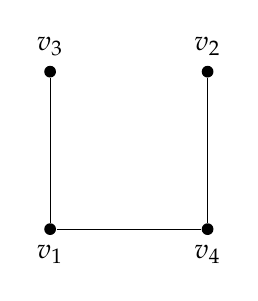
\begin{tikzpicture}

\node[circle, fill=black, inner sep=1.5pt, label=below:$v_{1}$] (v1) at (0,0) {};
\node[circle, fill=black, inner sep=1.5pt, label=above:$v_{2}$] (v2) at (2,2) {};
\node[circle, fill=black, inner sep=1.5pt, label=above:$v_{3}$] (v3) at (0,2) {};
\node[circle, fill=black, inner sep=1.5pt, label=below:$v_{4}$] (v4) at (2,0) {};
\draw (v2) -- (v4);
\draw (v1) -- (v3);
\draw (v1) -- (v4);

\end{tikzpicture}\end{center} 

A directed graph looks like this

\begin{center}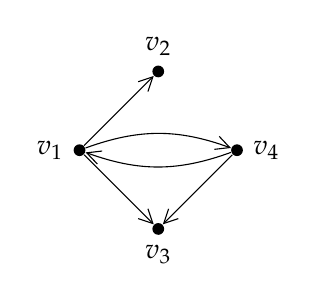
\begin{tikzpicture}

\node[circle, fill=black, inner sep=1.5pt, label=left:$v_{1}$] (v1) at (0,1) {};
\node[circle, fill=black, inner sep=1.5pt, label=above:$v_{2}$] (v2) at (1,2) {};
\node[circle, fill=black, inner sep=1.5pt, label=below:$v_{3}$] (v3) at (1,0) {};
\node[circle, fill=black, inner sep=1.5pt, label=right:$v_{4}$] (v4) at (2,1) {};

\draw[-{Straight Barb[length=5pt,width=5pt]}] (v1) edge[] node[right] {\LARGE $$} (v2);  
\draw[-{Straight Barb[length=5pt,width=5pt]}] (v1) edge[out=20,in=160] node[right] {\LARGE $$} (v4); 
\draw[-{Straight Barb[length=5pt,width=5pt]}] (v1) edge[] node[above] {$$} (v3);
\draw[-{Straight Barb[length=5pt,width=5pt]}] (v4) edge[out=200,in=340] node[above] {$$} (v1);
\draw[-{Straight Barb[length=5pt,width=5pt]}] (v4) edge[] node[above] {$$} (v3);

\end{tikzpicture}\end{center} 

Now, $E$ will be a set of ordered pairs: $E=\{(v_{1},v_{2}),(v_{1},v_{4}),(v_{1},v_{3}),(v_{4},v_{1}),(v_{4},v_{3})\}$.

\subsection*{Calc II Review}

Informally, a $\textbf{sequence}$ $\{a_{n}\}_{n=0}^{\infty}$ is
an indexed, infinitely long list of numbers.
\[
\{a_{n}\}_{n=0}^{\infty}=(a_{0},a_{1},a_{2},\dots)
\]

\begin{example} $a_{n}=1$ for all $n=0,1,2,3,\dots$. We can write
this as $\{1\}_{n=0}^{\infty}$.\end{example}

\begin{example} $a_{n}=n$ for all $n=0,1,2,3,\dots$. We can write
this as $\{n\}_{n=0}^{\infty}$.\end{example}

\begin{example} $a_{n}=n^{2}$ for all $n=0,1,2,3,\dots$. We can
write this as $\{n^{2}\}_{n=0}^{\infty}$.\end{example}

Alternatively, a $\textbf{sequence}$ $a_{n}$ is a function whose
domain is $\mathbb{N}$. 

\begin{example} The $\textbf{Fibonacci sequence}$ is defined recursively
as follows. Starting with $F_{0}=0$ and $F_{1}=1$, define $F_{n}=F_{n-1}+F_{n-2}$.\end{example}

\begin{example} $a_{n}=1$ for all $n=0,1,2,3,\dots$. We can write
this as $\{1\}_{n=0}^{\infty}$.\end{example}

\begin{defn} A $\textbf{partition}$ of $n$ is a ``way'' of writing
$n$ as a sum of positive integers where the order of the summands
is considered irrelevant. The $\textbf{partition function}$ $p(n)$
is the number of partitions of $n$.\end{defn}

$p(n)$ starts out as $1,1,2,3,5,7,11,15,\dots$. This sequence my
seem simple, but consider $p(200)=3972999029388$. 
\begin{center}
\begin{tabular}{c|c|c}
$n$ & partitions of $n$ & $p(n)$\tabularnewline
\hline 
$1$ & $1$ & $1$\tabularnewline
\hline 
$2$ & $2,\,1+1$ & $2$\tabularnewline
\hline 
$3$ & $3,\,1+2,\,1+1+1$ & $3$\tabularnewline
\hline 
$4$ & $4,\,1+3,\,2+2,\,1+1+2,\,1+1+1+1$ & $5$\tabularnewline
\end{tabular}
\par\end{center}

\subsection*{Generating Functions}

An extremely useful tool in combinatorics is the generating function
of a sequence.

\begin{defn}The (ordinary power series) $\textbf{generating function}$
for the sequence $\{a_{n}\}_{n=0}^{\infty}$ is the power series
\[
a_{0}+a_{1}x+a_{2}x^{2}+a_{3}x^{3}+\cdots=\sum_{n=0}^{\infty}a_{n}x^{n}.
\]

\end{defn}

\begin{example} The generating function for the sequence $\{1\}_{n=0}^{\infty}$
is
\[
\frac{1}{1-x}=1+x+x^{2}+\cdots
\]

\end{example}

\begin{example} The generating function for the sequence $\{\frac{1}{n!}\}_{n=0}^{\infty}$
is $e^{x}$. \end{example}

\begin{example} Let's calculate the generating function for $\{F_{n}\}_{n=0}^{\infty}$.
Let
\[
\mathcal{F}(x)=\sum_{n=0}^{\infty}F_{n}x^{n}.
\]

We have $x^{2}\mathcal{F}(x)-x\mathcal{F}(x)-\mathcal{F}(x)=-x$.
So
\[
\mathcal{F}(x)=\frac{x}{1-x-x^{2}}.
\]

\end{example}

\subsection*{A Recurrence Relation for $p(n)$.}

In the 1740's, Euler found the infinite product generating function
for $p(n)$:
\begin{align*}
\frac{1}{1-x}\cdot\frac{1}{1-x^{2}}\cdot\frac{1}{1-x^{3}}\cdots & =(1+x^{1}+x^{1+1}+x^{1+1+1}\cdots)(1+x^{2}+x^{2+2}+x^{2+2+2}\cdots)(1+x^{3}+x^{3+3}+x^{3+3+3}+\cdots)\cdots\\
 & =1+x^{1}+(x^{1+1}+x^{2})+(x^{1+1+1}+x^{1+2}+x^{3})+(x^{1+1+1+1}+x^{1+1+2}+x^{1+3}+x^{2+2}+x^{4})+\cdots\\
 & =1+x+2x^{2}+3x^{3}+5x^{4}\cdots\\
 & =\sum_{n=0}^{\infty}p(n)x^{n}.
\end{align*}
So Euler showed 
\begin{equation}
\prod_{n=0}^{\infty}\left(\frac{1}{1-x^{n}}\right)=\sum_{n=0}^{\infty}p(n)x^{n}.\label{eq:partitionprod}
\end{equation}

Later, he studied the reciprocal of the infinite product in (\ref{eq:partitionprod}
\begin{align}
(1-x)(1-x^{2})(1-x^{3})\cdots & =1-x-x^{2}+x^{5}+x^{7}-x^{12}-x^{15}+x^{22}+\cdots\label{eq:pentagonalprod}\\
 & =\sum_{j=-\infty}^{\infty}(-1)^{j}x^{\frac{3}{2}j^{2}-\frac{1}{2}j}\nonumber 
\end{align}

The integers occuring in the exponents on the righthand side of (\ref{eq:pentagonalprod})
are known as the pentagonal numbers. Euler found a recurrence of the
partition numbers as follows: 
\begin{align*}
1 & =\left(\frac{1}{1-x}\cdot\frac{1}{1-x^{2}}\cdot\frac{1}{1-x^{3}}\cdots\right)\left((1-x)(1-x^{2})(1-x^{3})\cdots\right)\\
 & =\left(p(0)+p(1)x+p(2)x^{2}+p(3)x^{3}+\cdots\right)\left(1-x-x^{2}+x^{5}+\cdots\right)\\
 & =\sum_{n=0}^{\infty}\left(p(n)-p(n-1)-p(n-2)+p(n-5)+\cdots\right)x^{n}
\end{align*}

It follows from this that 
\begin{equation}
p(n)=p(n-1)+p(n-2)-p(n-5)-\cdots.\label{eq:partitionrecurrence}
\end{equation}

\end{document}
